\documentclass[a4paper]{article}
\usepackage[utf8]{inputenc}
\usepackage[margin=2cm, top=1.5cm]{geometry}
\usepackage{tikz}
\usepackage{xcolor}
\usepackage{graphicx}
\usepackage{array}

% --- User Settings ----------------------------------------------------------
\newcommand{\InstitutionName}{Egypt University of Informatics}
\newcommand{\IDDigits}{14}        % Number of ID digits
\newcommand{\NumQuestions}{99}   % Total number of questions
\newcommand{\NumOptions}{8}      % Options per question  (max 8:  A-H)
\newcommand{\NumVersions}{26}    % Exam versions         (max 16: A-Z)

% --- Lengths (change once, applies everywhere) -------------------------------
\newcommand{\BubbleRcm}{0.22}     % bubble radius              (cm)
\newcommand{\BubbleStepCm}{0.6}  % horizontal bubble-to-bubble (cm)
\newcommand{\RowStepCm}{0.5}     % vertical row-to-row spacing (cm)
\newlength{\BubbleR}    \setlength{\BubbleR}{\BubbleRcm cm}
\newlength{\BubbleStep} \setlength{\BubbleStep}{\BubbleStepCm cm}
\newlength{\RowStep}    \setlength{\RowStep}{\RowStepCm cm}

% --- Colors -----------------------------------------------------------------
\colorlet{OMRColor}{magenta!40}   % drop-out color for scanner
\colorlet{MarkColor}{black}       % corner / timing mark color

% ----------------------------------------------------------------------------
\begin{document}
	\pagestyle{empty}
	
	% --- Corner & Timing Marks --------------------------------------------------
	\begin{tikzpicture}[remember picture, overlay]
		% Four corner marks: top-left is wider (2.0cm) to detect 180-degree rotation
		% Bottom markers adjusted to y=2.0 to maintain a safe margin from the page edge
		\foreach \anchor/\dx/\dy/\w in {
			north west/ 1.2/-1.2/2.0, % Top-Left (Wider for orientation)
			north east/-2.0/-1.2/0.8, % Top-Right
			south west/ 1.2/ 2.0/0.8, % Bottom-Left 
			south east/-2.0/ 2.0/0.8  % Bottom-Right 
		}{
			\fill[MarkColor]
			(current page.\anchor) ++(\dx cm, \dy cm)
			rectangle ++(\w cm, -0.8cm);
		}
		
		% Timing marks (left and right margins)
		\foreach \y in {0, \RowStepCm, ..., 22}{
			% Skip the first mark (y=0) so it doesn't merge with the bottom corner marks
			\ifdim \y pt > 0.1pt 
			% Left side
			\fill[MarkColor]
			(current page.south west) ++(1.2cm, 2cm + \y cm)
			rectangle ++(0.4cm, 0.2cm);
			% Right side (mirror)
			\fill[MarkColor]
			(current page.south east) ++(-1.6cm, 2cm + \y cm)
			rectangle ++(0.4cm, 0.2cm);
			\fi
		}
	\end{tikzpicture}
	
	% --- Top Row: Left = Info  |  Right = ID Bubbles ----------------------------
	\noindent
	%
	% -- Left block: logo + institution name + written fields (48% of width) ------
	\begin{minipage}[t]{0.48\textwidth}
		\vspace{0pt}
		\begin{center}
			
\includegraphics[width=4cm, height=1.2cm, keepaspectratio]{assets/logo}\\[3mm]
			{\large\bfseries \InstitutionName}\\[1mm]
			\rule{0.9\linewidth}{0.4pt}
		\end{center}
		\vspace{4mm}
		
		\renewcommand{\arraystretch}{1.8}
		\begin{tabular}{|p{0.22\linewidth}p{0.68\linewidth}|}
			\hline
			\textbf{Name:}       & \\[3mm] \hline
			\textbf{Course:}     & \\[3mm] \hline
			\textbf{Date:}       & \\[3mm] \hline
		\end{tabular}
	\end{minipage}%
	\hfill%
	% -- Right block: Student ID bubbles (48% of width) ---------------------------
	\begin{minipage}[t]{0.48\textwidth}
		\vspace{0pt}
		\raggedleft
		\textbf{Student ID:}\par\vspace{3mm}
		% Changed y to -\RowStep to match the vertical spacing of the rest of the sheet
		
\begin{tikzpicture}[x=\BubbleStep, y=-\RowStep]
			\foreach \col in {1,...,\IDDigits}{
				\draw[OMRColor,thick] (\col - 0.35, 0.4) rectangle (\col + 0.35, -0.4);
			}
		\end{tikzpicture}
		\par\vspace{1mm}
		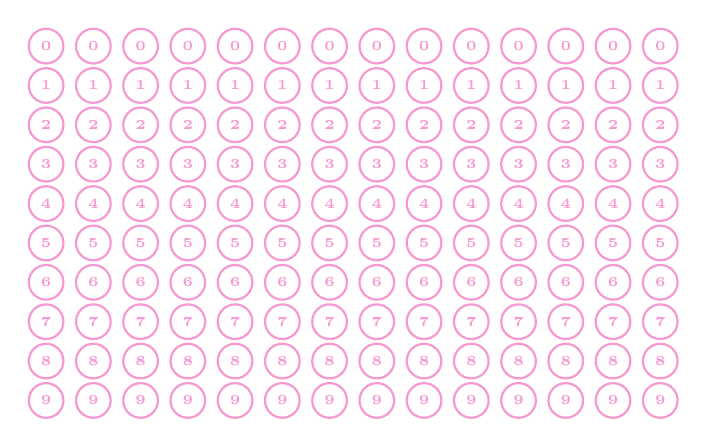
\begin{tikzpicture}[x=\BubbleStep, y=-\RowStep]
			\foreach \col in {1,...,\IDDigits}{
				\foreach \row in {0,...,9}{
					\draw[OMRColor, thick] (\col, \row) circle (\BubbleR)
					node[font=\tiny\bfseries, text=OMRColor] {\row};
				}
			}
		\end{tikzpicture}
	\end{minipage}
	
	% --- Bottom Row: Exam Version (full width) -----------------------------------
	\vspace{3mm}
	\noindent
	\textbf{Exam Version:}\par\vspace{3mm}
	\noindent
	
\begin{tikzpicture}[x=\BubbleStep, y=0cm]
		\foreach \v [count=\i] in {A,B,C,D,E,F,G,H,I,J,K,L,M,N,O,P,Q,R,S,T,U,V,W,X,Y,Z}{
			\ifnum\i>\NumVersions\else
			\draw[OMRColor, thick] (\i, 0) circle (\BubbleR)
			node[font=\tiny\bfseries, text=OMRColor] {\v};
			\fi
		}
	\end{tikzpicture}
	
	\noindent\rule{\linewidth}{0.6pt}
	\vspace{-2mm}
	
	% --- Answers Section (3 columns) --------------------------------------------
	\noindent\hspace*{-0.2cm}%
	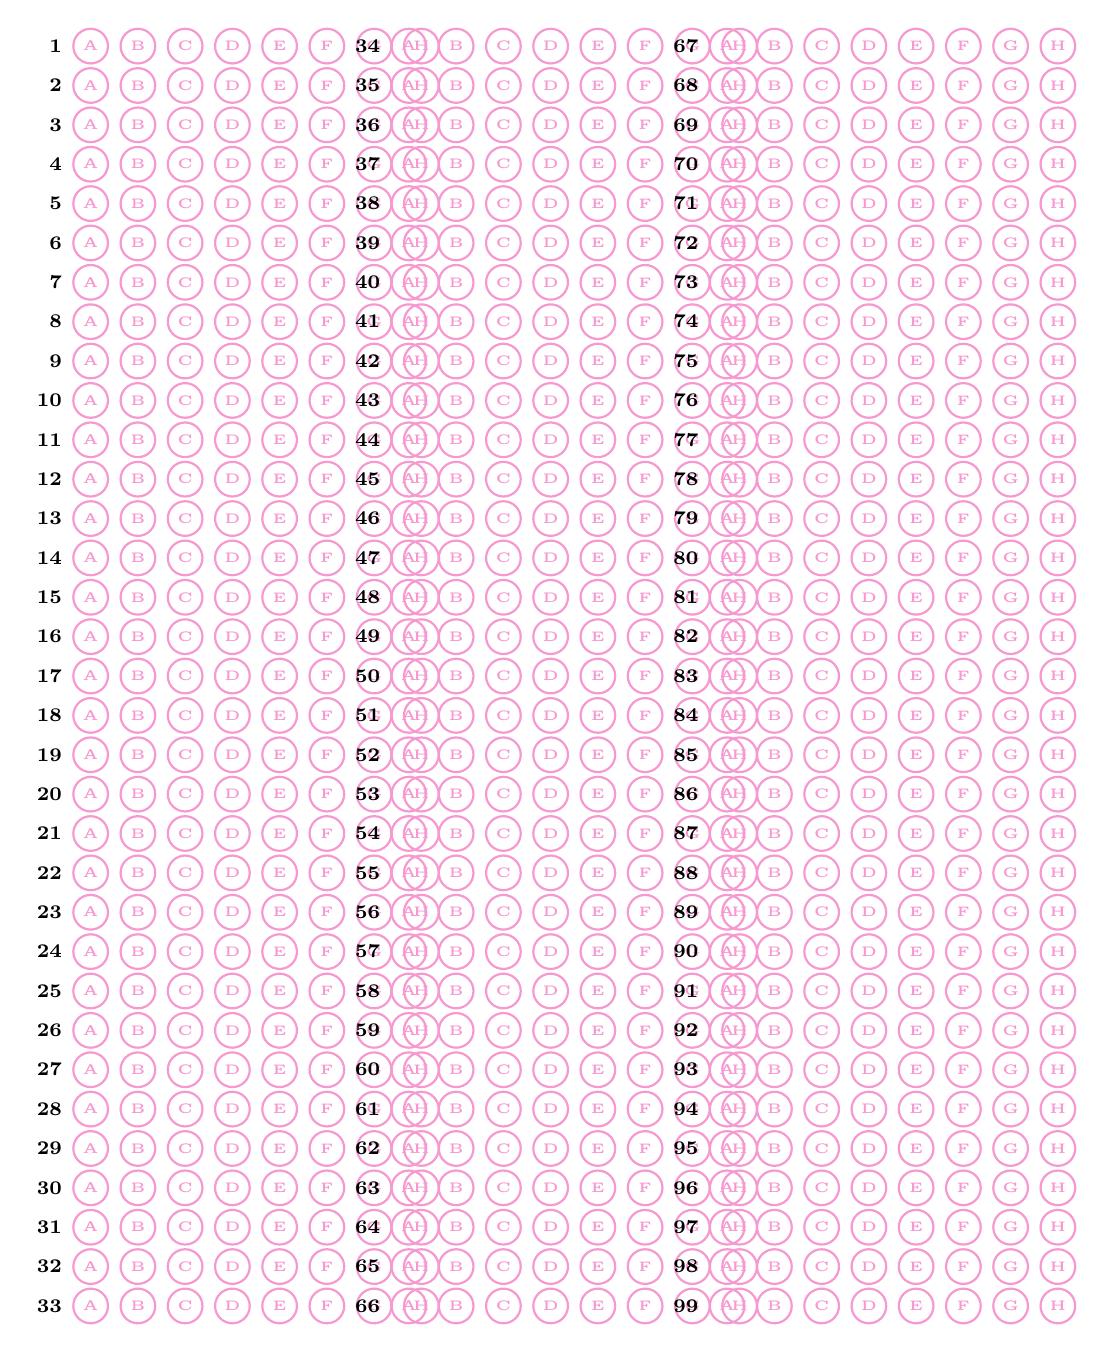
\begin{tikzpicture}[x=\BubbleStep, y=-\RowStep]
		\pgfmathtruncatemacro{\RowsPerCol}{ceil(\NumQuestions/3)}
		\pgfmathsetmacro{\ColWidth}{\the\linewidth / \the\BubbleStep / 3}
		
		\foreach \q in {1,...,\NumQuestions}{
			\pgfmathtruncatemacro{\colIdx}{(\q-1)/\RowsPerCol}
			\pgfmathtruncatemacro{\rowIdx}{mod(\q-1,\RowsPerCol)}
			\pgfmathsetmacro{\xOff}{\colIdx * \ColWidth}
			
			\node[anchor=east, font=\scriptsize\bfseries] at (\xOff + 1.2, \rowIdx) {\q};
			
			\foreach \opt [count=\i] in {A,B,C,D,E,F,G,H}{
				\ifnum\i>\NumOptions\else
				\draw[OMRColor, thick]
				(\xOff + 0.6 + \i, \rowIdx) circle (\BubbleR)
				node[font=\tiny\bfseries, text=OMRColor] {\opt};
				\fi
			}
		}
	\end{tikzpicture}
	
\end{document}